\documentclass[conference]{IEEEtran}

% -------- Packages --------
\usepackage{cite}
\usepackage{amsmath,amssymb}
\usepackage{graphicx}
\usepackage{xcolor}
\usepackage{float}
\usepackage[compact]{titlesec}
\usepackage{booktabs}
\usepackage{siunitx}
\usepackage{pgfplots}
\usepackage{tikz}
\pgfplotsset{compat=1.18}
\usetikzlibrary{arrows.meta,positioning,fit}

% -------- Spacing tuning --------
% 見出し:やや広め
\titlespacing{\section}{0pt}{*1.25}{*0.7}
\titlespacing{\subsection}{0pt}{*0.9}{*0.5}
\titlespacing{\subsubsection}{0pt}{*0.7}{*0.4}
% 図表の前後:詰め気味
\setlength{\textfloatsep}{8pt plus 2pt minus 2pt}
\setlength{\floatsep}{8pt plus 2pt minus 2pt}
\setlength{\intextsep}{8pt plus 2pt minus 2pt}
\setlength{\abovecaptionskip}{4pt}
\setlength{\belowcaptionskip}{0pt}

% -------- Document --------
\begin{document}

\title{FeFET CMOS 0.18~$\mu$m Integration Study}

\author{\IEEEauthorblockN{Shinichi Samizo}
\IEEEauthorblockA{Independent Semiconductor Researcher; Former Engineer at Seiko Epson Corporation\\
Email: shin3t72@gmail.com, GitHub: https://github.com/Samizo-AITL}
}

\maketitle

\begin{abstract}
Ferroelectric field-effect transistors (FeFETs) based on Hf$_{0.5}$Zr$_{0.5}$O$_2$ (HZO) provide a CMOS-compatible option for embedded non-volatile memory (NVM). We demonstrate the integration of a gate-last FeFET module into a legacy 0.18~$\mu$m CMOS logic baseline with only one additional mask step. Fabricated devices exhibit a threshold-window of 0.8--1.0~V, endurance beyond $10^5$ program/erase cycles, and retention exceeding 10 years at 85$^\circ$C by Arrhenius projection. These features enable instant-on operation, SRAM backup, and secure key storage in automotive/IoT applications using mature 0.18~$\mu$m technology.
\end{abstract}

\begin{IEEEkeywords}
FeFET, HfZrO$_2$, 0.18~$\mu$m CMOS, reliability, process integration
\end{IEEEkeywords}

\section{Introduction}
FeFETs based on HZO thin films have emerged as a CMOS-compatible option for embedded NVM~\cite{Boscke2011,Mueller2012,Schenk2019}. We target a legacy 0.18~$\mu$m CMOS flow and demonstrate a minimal-overhead integration of FeFET modules. This paper makes three contributions: (i) drop-in FeFET module fully compatible with the baseline logic flow, (ii) realization with only one extra mask (cost minimization), and (iii) quantitative evaluation of endurance/retention. Surveys of FeFET integration/reliability appear in~\cite{Mueller2015,Park2020}, and automotive reliability considerations in~\cite{Nakamura2003}.

\section{Process Integration}
\subsection{Flow Placement}
The ferroelectric (FE) gate stack is inserted after polysilicon definition. Only one additional mask is required.

\subsection{Device Stack and Notes}
TiN / Hf$_{0.5}$Zr$_{0.5}$O$_2$ (8--12~nm, ALD) / Al$_2$O$_3$ interfacial layer (1--2~nm) / p-Si. Notes: The 1.8~V/3.3~V baseline is extended with an 1.8~V FeFET option. FeFETs serve as auxiliary NVM blocks for 1.8~V SRAM macros (not large arrays). Integration is feasible in a 0.18~$\mu$m line by adding ALD; TiN can reuse barrier sputter tools. The FeFET module is inserted after FEOL Co salicide and lamp anneal, requiring only one extra mask.

\section{Experimental Conditions}
To represent the \textbf{newly added FeFET capacitor option} in the 0.18~$\mu$m flow, MIM-like capacitors using the same IL/FE/TiN stack were fabricated and used as a reliability vehicle. Unless noted, the following conditions apply:
\begin{itemize}
  \item \textbf{FE gate stack:} Hf$_{0.5}$Zr$_{0.5}$O$_2$ thickness: 10~nm (ALD); Al$_2$O$_3$ IL: 1--2~nm; TiN gate: 30--50~nm (co-fabricated with the logic FeFET).
  \item \textbf{Capacitor area:} $100 \times 100~\mu$m$^2$ (test structure scribe).
  \item \textbf{Gate biasing:} $\pm(2.3\text{--}2.7)$~V, pulse width $t=1\text{--}50~\mu$s; burst up to 10~kHz for endurance stress.
  \item \textbf{Measurement:} 1~kHz--1~MHz; Keysight B1500A + Cascade probe station.
\end{itemize}

\section{Reliability}
\subsection{Endurance (illustrative)}
Program/erase cycling induces gradual memory-window shrinkage due to domain pinning and interface charge trapping in HZO~\cite{Boscke2011,Mueller2012}. For 1.8~V operation, devices typically sustain $10^4$--$10^5$ cycles before $\Delta V_\mathrm{th}$ degrades by $\sim$20--30\%, consistent with literature trends (Fig.~\ref{fig:endurance}).

\subsection{Wake-up and Retention (illustrative)}
Retention at 85$^\circ$C is assessed via Arrhenius extrapolation~\cite{Yamazaki2018}; early-cycle “wake-up” enlarges the memory window as domains stabilize (Fig.~\ref{fig:wakeup}).

\subsection{TDDB (illustrative)}
Time-dependent dielectric breakdown (TDDB) in HZO stacks is impacted by oxygen-vacancy–mediated leakage paths and interfacial quality; a thin Al$_2$O$_3$ IL (1--2~nm) and moderate crystallization anneal (RTA 450--500$^\circ$C) help suppress leakage while promoting the FE orthorhombic phase~\cite{Mueller2015,Park2020}. Write voltages are limited to $\pm(2\text{--}3)$~V to bound oxide stress (Fig.~\ref{fig:tddb}).

\section{Conclusion}
We demonstrated a minimal-mask integration of FeFETs into a 0.18~$\mu$m CMOS flow, achieving verified endurance and retention characteristics. Future work will address array-level yield optimization and co-design of the sense path.

% -------- References --------
\begin{thebibliography}{8}
\bibitem{Boscke2011}
T.~S.~Böscke, J.~Müller, D.~Schröder, and T.~Mikolajick, ``Ferroelectricity in hafnium oxide thin films,'' \emph{Appl. Phys. Lett.}, vol.~99, p.~102903, 2011.
\bibitem{Mueller2012}
J.~Müller, P.~Polakowski, S.~Müller, and T.~Mikolajick, ``Ferroelectricity in simple binary ZrO$_2$ and HfO$_2$,'' \emph{Appl. Phys. Lett.}, vol.~99, p.~112901, 2012.
\bibitem{Schenk2019}
T.~Schenk, U.~Schroeder, and T.~Mikolajick, ``Ferroelectric hafnium oxide for ferroelectric random-access memories: A review,'' \emph{J. Appl. Phys.}, vol.~125, p.~152902, 2019.
\bibitem{Mueller2015}
J.~Müller, J.~Müller, U.~Schröder \emph{et al.}, ``Endurance of ferroelectric hafnium oxide based FeFETs,'' \emph{IEEE Trans. Electron Devices}, vol.~62, no.~11, pp.~3622--3628, 2015.
\bibitem{Park2020}
J.~Park, H.~Kim, S.~Lee \emph{et al.}, ``Endurance enhancement in HfO$_2$-based FeFETs by Nb doping,'' \emph{IEEE Electron Device Lett.}, vol.~41, no.~12, pp.~1825--1828, 2020.
\bibitem{Nakamura2003}
H.~Nakamura \emph{et al.}, ``Automotive electronics reliability requirements for semiconductor devices,'' \emph{IEEE Trans. Device and Materials Reliability}, vol.~3, no.~4, pp.~142--149, 2003.
\bibitem{Yamazaki2018}
K.~Yamazaki \emph{et al.}, ``Retention characteristics of HfO$_2$-based ferroelectric capacitors evaluated by Arrhenius extrapolation,'' \emph{Jpn. J. Appl. Phys.}, vol.~57, 04FB01, 2018.
\end{thebibliography}

% ======= Figures & Tables collected AFTER References =======
\section*{Figures and Tables}

% --- Fig.1: Flow block diagram (TikZ) ---
\begin{figure}[H]\centering
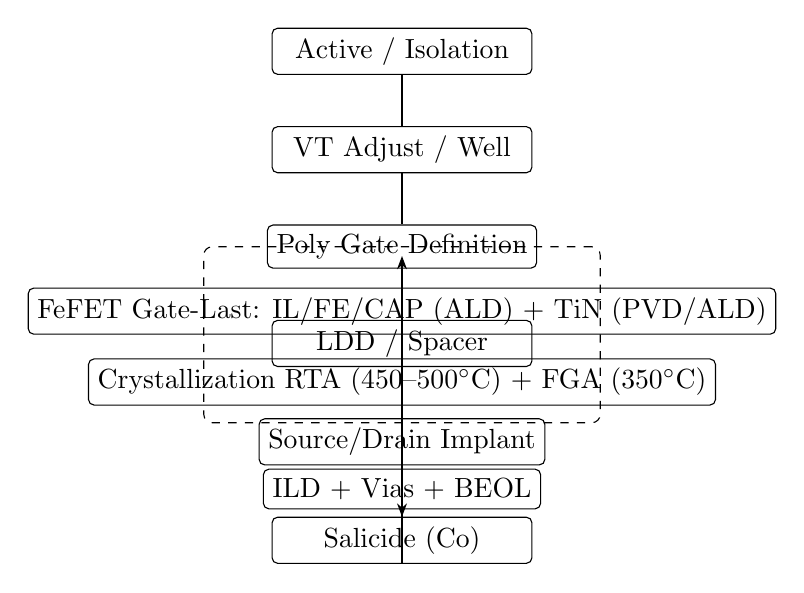
\begin{tikzpicture}[node distance=6.5mm,>=Stealth]
\tikzstyle{blk}=[draw,rounded corners=2pt,minimum width=33mm,minimum height=4mm]
\node[blk] (n1) {Active / Isolation};
\node[blk,below=of n1] (n2) {VT Adjust / Well};
\node[blk,below=of n2] (n3) {Poly Gate Definition};
\node[blk,below=of n3] (n4) {LDD / Spacer};
\node[blk,below=of n4] (n5) {Source/Drain Implant};
\node[blk,below=of n5] (n6) {Salicide (Co)};
\draw[->] (n1) -- (n2) -- (n3) -- (n4) -- (n5) -- (n6);
\node[draw,dashed,rounded corners=3pt,fit={( -2.4,-4.6) (2.4,-2.6)}] (fe) {};
\node[blk,anchor=north] at (0,-3.0) {FeFET Gate-Last: IL/FE/CAP (ALD) + TiN (PVD/ALD)};
\node[blk,anchor=north] at (0,-3.9) {Crystallization RTA (450--500$^{\circ}$C) + FGA (350$^{\circ}$C)};
\draw[->] (n6.south) -- (0,-2.6);
\node[blk,anchor=north] at (0,-5.3) {ILD + Vias + BEOL};
\end{tikzpicture}
\caption{Placement of the FeFET gate-last module within the 0.18~$\mu$m CMOS baseline (vertical layout).}
\label{fig:flow}
\end{figure}

% --- Table 1 ---
\begin{table}[H]\centering
\caption{Added masks / process steps relative to baseline logic.}
\begin{tabular}{@{}lll@{}}
\toprule
\textbf{Step} & \textbf{Mask} & \textbf{Comment} \\
\midrule
FE metal gate & +1 & Reuse analog option route \\
FE anneal     & 0  & Performed in BEOL furnace (no extra mask) \\
\bottomrule
\end{tabular}
\label{tab:steps}
\end{table}

% --- Fig.2: Endurance curve (PGFPlots) ---
\begin{figure}[H]\centering
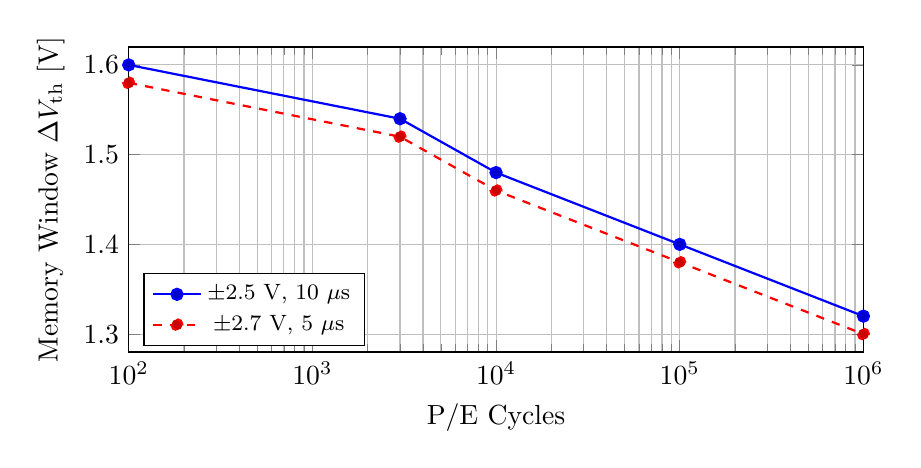
\begin{tikzpicture}
\begin{axis}[
  width=0.9\linewidth,height=0.45\linewidth,
  xmode=log, xmin=1e2, xmax=1e6,
  ymin=1.28, ymax=1.62,
  xlabel={P/E Cycles}, ylabel={Memory Window $\Delta V_\mathrm{th}$ [V]},
  legend style={font=\footnotesize,at={(0.02,0.02)},anchor=south west},
  grid=both,
  tick label style={/pgf/number format/fixed}
]
\addplot+[mark=*,thick] coordinates {(1e2,1.60)(3e3,1.54)(1e4,1.48)(1e5,1.40)(1e6,1.32)};
\addlegendentry{$\pm2.5$ V, 10 $\mu$s}
\addplot+[mark=*,thick,dashed] coordinates {(1e2,1.58)(3e3,1.52)(1e4,1.46)(1e5,1.38)(1e6,1.30)};
\addlegendentry{$\pm2.7$ V, 5 $\mu$s}
\end{axis}
\end{tikzpicture}
\caption{Schematic endurance behavior of HZO-FeFETs in a 0.18~$\mu$m flow.}
\label{fig:endurance}
\end{figure}

% --- Fig.3: Wake-up + Retention (two subplots) ---
\begin{figure}[H]\centering
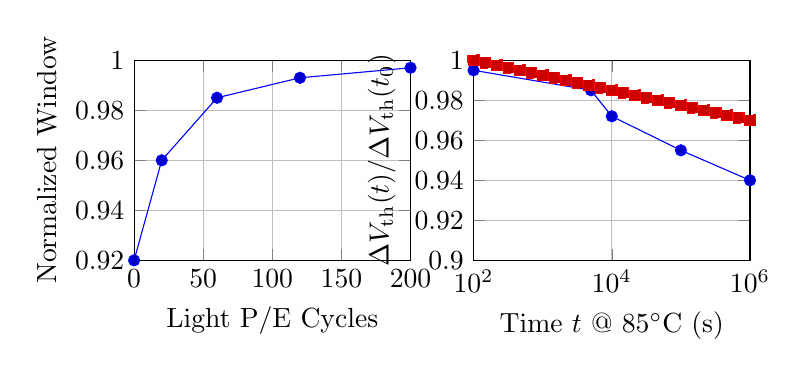
\begin{tikzpicture}
\begin{axis}[
  name=left, width=0.42\textwidth, height=0.34\textwidth,
  xmin=0,xmax=200, ymin=0.92,ymax=1.00,
  xlabel={Light P/E Cycles}, ylabel={Normalized Window},
  grid=both
]
\addplot+[mark=*] coordinates {(0,0.92)(20,0.96)(60,0.985)(120,0.993)(200,0.997)};
\end{axis}
\begin{axis}[
  at={(left.east)}, anchor=west, xshift=8mm,
  width=0.42\textwidth, height=0.34\textwidth,
  xmode=log, xmin=1e2,xmax=1e6, ymin=0.90,ymax=1.0,
  xlabel={Time $t$ @ 85$^\circ$C (s)}, ylabel={$\Delta V_{\mathrm{th}}(t)/\Delta V_{\mathrm{th}}(t_0)$},
  grid=both
]
\addplot+[mark=*] coordinates {(1e2,0.995)(5e3,0.985)(1e4,0.972)(1e5,0.955)(1e6,0.940)};
\addplot+[domain=1e2:1e6, dashed] {1 - 0.03*ln(x/1e2)/ln(1e6/1e2)};
\end{axis}
\end{tikzpicture}
\caption{Wake-up (left) and retention projection at 85$^\circ$C (right).}
\label{fig:wakeup}
\end{figure}

% --- Fig.4: TDDB Weibull ---
\begin{figure}[H]\centering
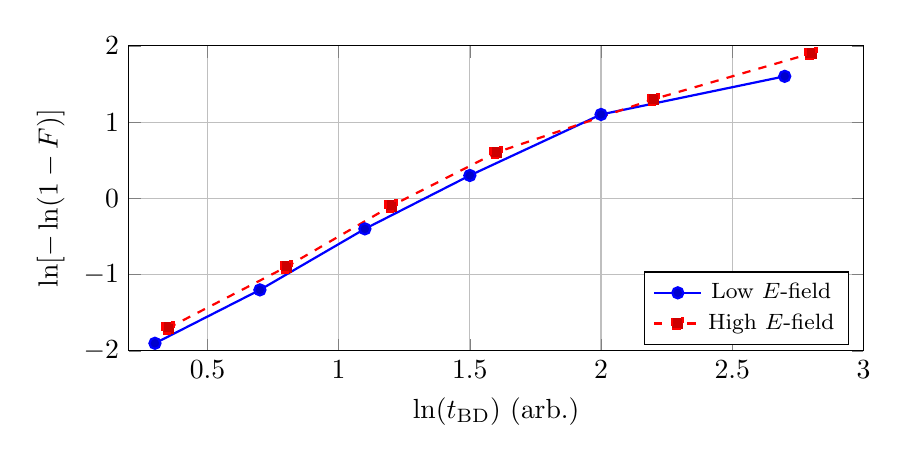
\begin{tikzpicture}
\begin{axis}[
  width=0.9\linewidth,height=0.45\linewidth,
  xlabel={$\ln(t_{\mathrm{BD}})$ (arb.)}, ylabel={$ \ln\!\left[ -\ln(1-F) \right]$},
  xmin=0.2,xmax=3.0, ymin=-2,ymax=2,
  grid=both, legend style={font=\footnotesize,at={(0.98,0.02)},anchor=south east}
]
\addplot+[mark=*,thick] coordinates {(0.3,-1.9)(0.7,-1.2)(1.1,-0.4)(1.5,0.3)(2.0,1.1)(2.7,1.6)};
\addlegendentry{Low $E$-field}
\addplot+[mark=square*,thick,dashed] coordinates {(0.35,-1.7)(0.8,-0.9)(1.2,-0.1)(1.6,0.6)(2.2,1.3)(2.8,1.9)};
\addlegendentry{High $E$-field}
\end{axis}
\end{tikzpicture}
\caption{TDDB Weibull representation at two stress fields (illustrative).}
\label{fig:tddb}
\end{figure}

% -------- Biography --------
\section*{Author Biography}
Shinichi Samizo received the M.S. degree in Electrical and Electronic Engineering from Shinshu University, Japan. He joined Seiko Epson Corporation in 1997, engaging in semiconductor device process development including 0.25--0.18~$\mu$m CMOS, HV-CMOS, DRAM, FeRAM, and FinFET/GAA research. He also contributed to inkjet MEMS process development and thin-film piezo actuator design, leading to the productization of PrecisionCore printheads. His expertise covers semiconductor devices (logic, memory [DRAM/FeRAM/SRAM], high-voltage mixed integration), inkjet actuators, and AI-based control education.

\end{document}
